% !TeX spellcheck = ru_RU
% !TEX root = vkr.tex

\section{Тестирование транслятора}

\begin{figure}[h]
    \begin{center}
        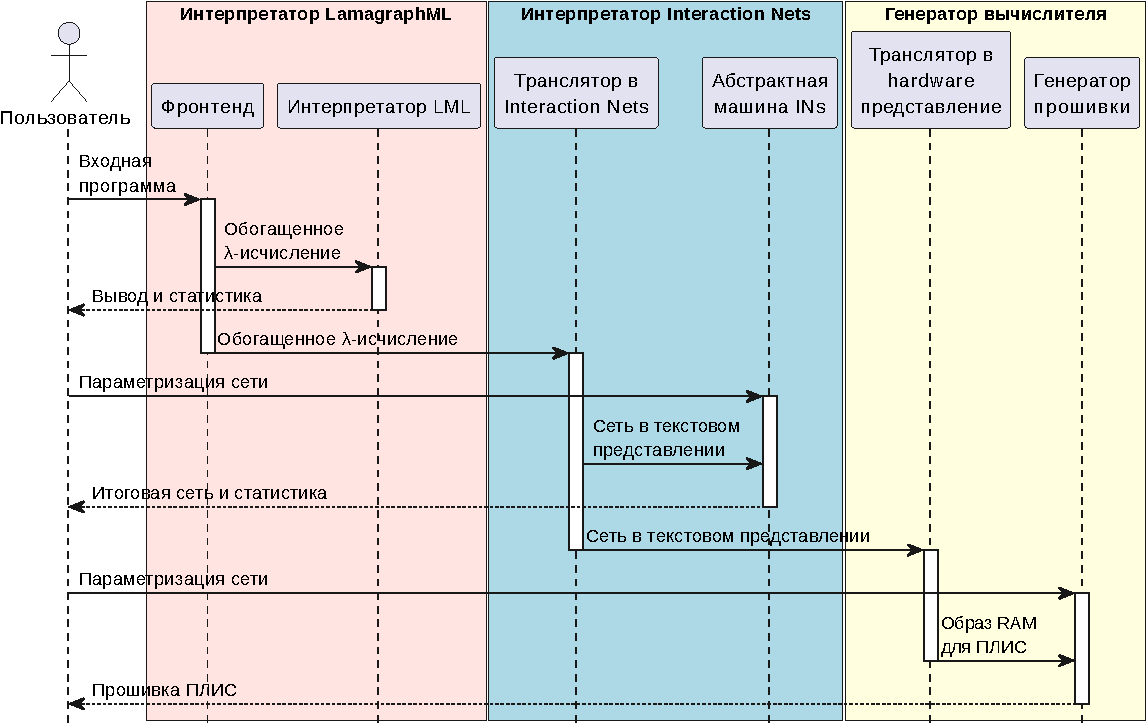
\includegraphics[width=0.9\linewidth]{using.pdf}
    \end{center}
    \caption{Диаграмма взаимодействия пользователя с программно-аппаратным стеком Lamagraph.}
    \label{fig:using}
\end{figure}

На данном этапе развития проекта проведение сравнительных экспериментов невозможно, тем не менее пользователь уже может взаимодействовать с инструментом.

Так, передав на вход программу на \LamagraphML{} пользователь может получить вывод интерпретатора, а также вывод абстрактной машины и соответствующую статистику, что проиллюстрировано на рисунке~\ref{fig:using}.

\todo[inline]{Дальше сюда нужно будет написать что-то типа: "Мы написали k лямбда-термов на LML, загнали их в стек и получили что-то".
    Что? Вариант 1: не смотреть на интерпретатор LML, а просто взять правила для абстрактной машины и посмотреть разницу с одним/множеством токенов.
    Вариант 2: научиться выдёргивать результат исполнения из интерпретатора LML и сравнивать его с итоговой сетью.
    Вариант 1 мне кажется проще и понятнее сейчас. Потому что сравнивать два разных прелдставления глазами сложно, плюс я не очень понимаю, что за дичь я смогу вынуть из интерпретатора.}
